% Example to generate the coverpages of a PhD thesis with PhDcover.sty
% Please contact the TeX support team when experiencing problems.
% This file produces a 125% size (to be reduced by 80%),
% as is customary with the text pages as well.
%
\documentclass[12pt,makeidx]{phdthesis}
\usepackage{a4wide}
\usepackage{listings}
\usepackage{palatino}

\usepackage{makeidx}
\makeindex

\usepackage{natbib}
\usepackage{fancyheadings}
\usepackage{amsmath}
\usepackage{amssymb}
\usepackage{epsfig}
\usepackage{subfigure}
\usepackage{graphics}
\usepackage{float}
%\usepackage[abbr]{harvard}
\usepackage{rotating}
\usepackage{multirow}
\usepackage{comment}
\usepackage{captionhack}
\usepackage{epigraph}
\usepackage{footnote}
\usepackage[sectionbib]{chapterbib} 
%\usepackage[rootbib]{chapterbib} 

\renewcommand{\textfraction}{0.01}
\renewcommand{\topfraction}{0.99}
\renewcommand{\floatpagefraction}{0.99}
\renewcommand{\bottomfraction}{0.99}

\makesavenoteenv{tabular} 

\newenvironment{Abstract}
{\begin{center}\textbf{Abstract}%
 \end{center} \small \it \begin{quote}}
{\end{quote}}

\begin{document}
\title{RegaDB v2.0 Installation Manual}
\author{Pieter Libin\\mybiodata, Biomedical IT Solutions}
\maketitle

\cleardoublepage
\lhead[]{\fancyplain{}{\rightmark}}
\chead[\fancyplain{}{}]{\fancyplain{}{}}
\rhead[\fancyplain{}{\leftmark}]{\fancyplain{}{}}
%\rhead[\fancyplain{}{}]{\fancyplain{}{}}
%\lhead[\fancyplain{}{}]{\fancyplain{}{}}

\setcounter{tocdepth}{2}
\tableofcontents

%%  add the acknowledgements to the table of contents
%\cleardoublepage
\addcontentsline{toc}{chapter}{Acknowledgements}
%\include{thesis_acknowledgements}

\cleardoublepage

%%% Customisation of the header and footer for the chapters
%\pagestyle{headings}
%------------------------------
\newcommand{\publ}{}

\pagestyle{fancyplain}
\renewcommand{\sectionmark}[1]{\markright{\it \thesection.\ #1}}
\renewcommand{\chaptermark}[1]{\markboth{
       \it \thechapter.\ #1}{}}
\lhead[\thepage]{\fancyplain{\publ}{\rightmark}}
\chead[\fancyplain{}{}]{\fancyplain{}{}}
\rhead[\fancyplain{}{\leftmark}]{\fancyplain{}{\thepage}}
\lfoot[]{}
\cfoot[]{}
\rfoot[]{}

%------------------------------
\pagenumbering{arabic}

\chapter{Introduction}
\label{chapter:introduction}

\section{General Introduction}

RegaDB is a server side Java2 application, which runs in a Servlet Container (eg. Tomcat). For data storage RegaDB relies on a RDBMS. Clients can access the RegaDB by browsing to the machine where the server software is installed, any popular browser can be used (Mozilla Firefox, Microsoft Internet Explorer).

Currently we support both Microsoft Windows and Linux operating systems. These platforms are officially tested, but any other platform which meets our requirements should be able to run RegaDB.

\section{Revision}
23 August 2007: Initial creation
\\
9 May 2009: Update for RegaDB v2.0
\\
16 Februari 2011: Update

\section{System requirements}
Microsoft Windows 2000 or higher or a Linux distribution configured with the following software:
\begin{itemize}
\item Sun Java2 Standard Edition version 5.0 or higher
\item Apache Tomcat Core 6 or higher
\item Postgresql 8.2.4 or higher
\end{itemize}

\chapter{Guided auto-install}
\label{chapter:auto-install}

\section{Introduction}
Download the latest regadb-install.exe installation executable from the RegaDB website. Doubleclick the executable and the installer startup screen will appear.

\section{Stepping through the automatic installer}
\subsection{Acknowledge the license}
This page asks you to read the RegaDB license, which is the GNU Public License (GPLv2). Briefly, this license
provides you the right to use the software in any way you like, and
grants you the right to access and modify the underlying source code.

You may distribute the software further, provided that you keep the
license intact, and that you also give access to the source code (in
case made modifications).

You should be aware that the software comes with no warranty. 
\\
\vspace{0.5cm}~ \\ \centerline{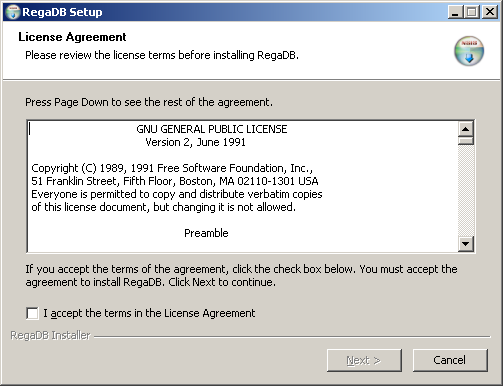
\includegraphics[width=8cm] {pics/nsis/license_agreement_1.png}}
\\
If you agree with the license enable the checbox and click \textbf{Next}.
\vspace{0.5cm}~ \\ \centerline{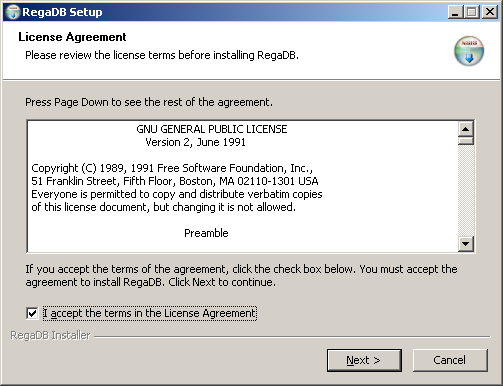
\includegraphics[width=8cm] {pics/nsis/license_agreement_2.png}}

\subsection{Select components to install}
Select all the modules for a completely automatic installation (default). Click \textbf{Next}.
\\\textit{If you only install the core module, some manual steps will be necessary after the guided installation procedure.}
\\
\vspace{0.5cm}~ \\ \centerline{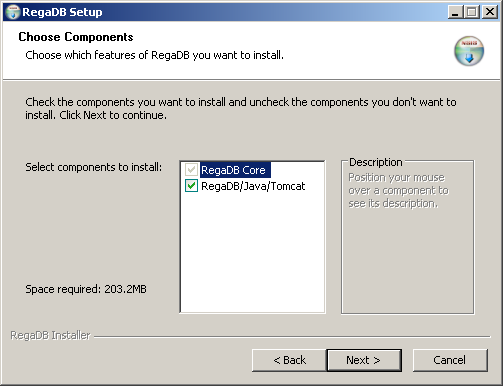
\includegraphics[width=8cm] {pics/nsis/select_components_3.png}}

\subsection{Specify the installation path}
The default installation path is preselected, if you agree with this installation path, please click \textbf{Next}.
\\
\vspace{0.5cm}~ \\ \centerline{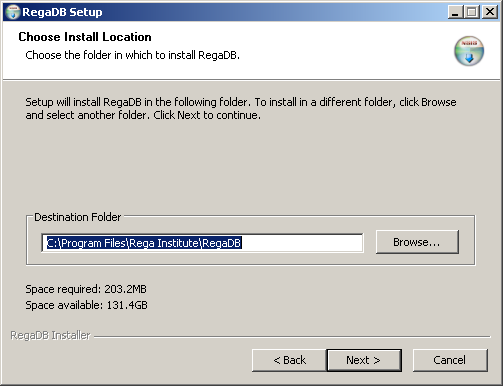
\includegraphics[width=8cm] {pics/nsis/installation_path_4.png}}
If you wish to have another installation path, click \textbf{Browse...} and select the appropriate installation directory.
\\
\vspace{0.5cm}~ \\ \centerline{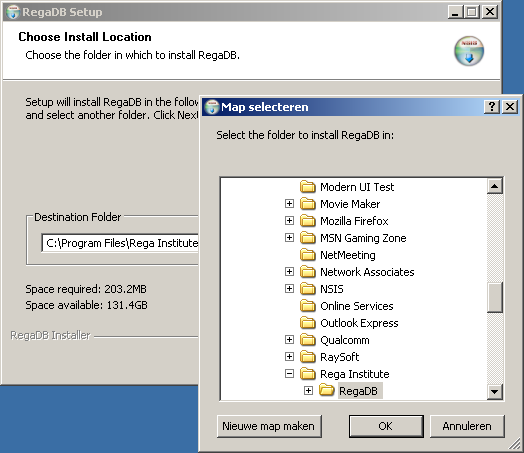
\includegraphics[width=8cm] {pics/nsis/installation_path_5.png}}


\subsection{Select the RDBMS to be used by RegaDB}
Please select the default database, this will enable RegaDB to use the Java RDBMS Hsqldb, than click \textbf{Next}.
\\
\vspace{0.5cm}~ \\ \centerline{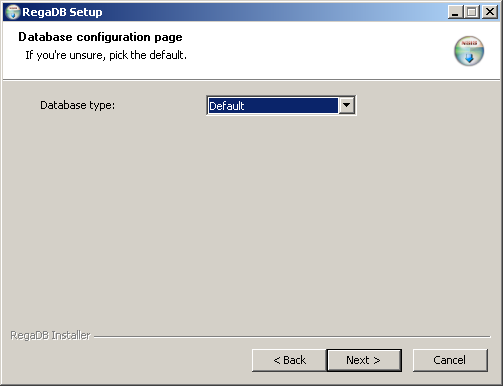
\includegraphics[width=8cm] {pics/nsis/select_database_6.png}}
\textit{If you select Postgresql in this page, further manual steps will be necessary.}

\subsection{Provide http proxy information}
While using RegaDB, the software requires internet access. Therefore, if your internet connection requires the use of a proxy, fill in your proxy settings. If you have a direct internet connection you may skip this step.
\\
\vspace{0.5cm}~ \\ \centerline{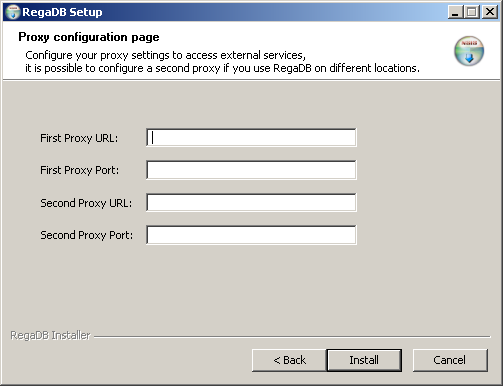
\includegraphics[width=8cm] {pics/nsis/select_proxy_7.png}}
Fill in your settings, and click \textbf{Next}. 
\\
\vspace{0.5cm}~ \\ \centerline{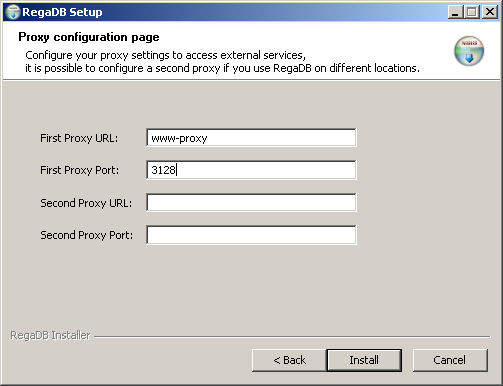
\includegraphics[width=8cm] {pics/nsis/select_proxy_8.png}}
RegaDB supports multiple proxy settings, and allows you to select the appropriate settings when you log in to the system.

\subsection{Installing the software}
Once all the configuration steps have been done, the software will be installed.
\\
\vspace{0.5cm}~ \\ \centerline{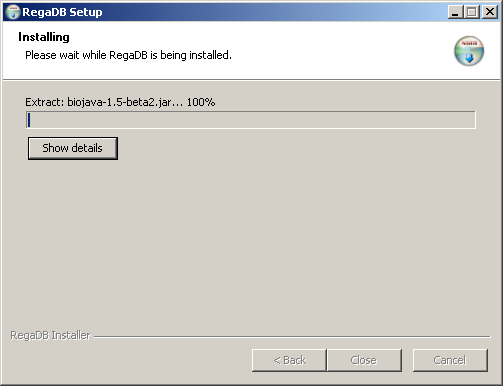
\includegraphics[width=8cm] {pics/nsis/installing_9.png}}
When the installation is complete, click \textbf{Close}. 
\\
\vspace{0.5cm}~ \\ \centerline{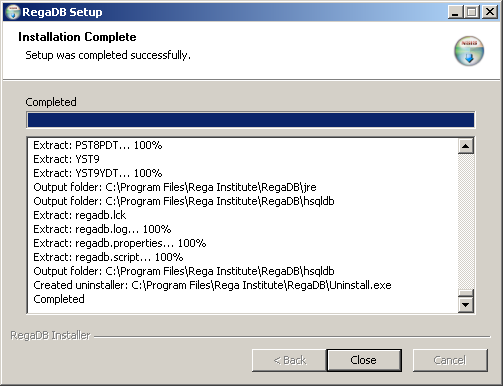
\includegraphics[width=8cm] {pics/nsis/installing_10.png}}
\\Please proceed to the Post installation chapter to finish the configuration of RegaDB (chapter~\ref{chapter:post_install}).

\chapter{Manual installation}
\label{chapter:manual_install}

\section{Introduction}
The manual installation can be done on both Microsoft Windows 2000 or higher or a Linux distribution with the following software pre-installed : 
\begin{itemize}
\item Sun Java2 Standard Edition version 5.0 or higher
\item Apache Tomcat Core 5.5 or higher (other Servlet containers might work, but are not officially supported yet)
\item Postgresql 8.2.4 or higher
\end{itemize}
If you have no experience installing this software, please consult your local system administor.

\section{Manual installation steps}
\subsection{Obtaining the RegaDB software package}
The RegaDB v2.0 software package can be downloaded from our website. The regadb-package.zip (Microsoft Windows) or regadb-package.tgz (Linux) contains all necessary files to perform a manual installation of the RegaDB software.

\subsection{Configuring the Postgresql database}
Log in as posgres administrator to psql
\\
\\
Create a new role:
\\
\textbf{create user \textit{role\_name} password '\textit{role\_password}';}
\\
\\
Create a new database:
\\
\textbf{create database regadb owner \textit{role\_name};}
\\
\\
Create the schema:
\\
\textbf{create schema regadbschema authorization \textit{role\_name};}
\\
\\
Log out from psql
\\
\\
Create the Postgres database structure (this file is part of the RegaDB software package)
\\
\textbf{psql -U \textit{role\_name} regadb -f posgresSchema.sql}

\subsection{RegaDB configuration}
RegaDB requires a XML configuration file, a documented example file is available in the RegaDB software package (global-conf.xml). This config file can be placed at the default location (/etc/rega\_institute/regadb), or at an alternative location.

If you place the configuration file at an alternative location, you should define an environment variable called \textbf{REGADB\_CONF\_DIR} containing this path.
Following attributes of the XML file should be filled in:
\begin{itemize}
\item hibernate.connection.driver\_class : the default value is correct, do not change this
\item hibernate.connection.password : replace default by your \textit{role\_password}
\item hibernate.connection.url : replace default by the URL of your Postgresql database + /regadb (eg. jdbc:postgresql://serverName:5432/regadb)
\item hibernate.connection.username : replace default by your \textit{role\_name}
\item hibernate.dialect : the default value is correct, do not change this
\item regadb.query.resultDir : replace default by a directory where query results should be stored (eg. /soft/regadb/queryResults), this directory should be writable by your servlet container
\item http.proxy.url : replace default by your proxy server name, if you have direct access to internet, simply remove default
\item http.proxy.port : replace default by your proxy server port, if you have direct access to internet, simply remove default
\end{itemize}

Note that this file should only be accessible by your servlet container, so please make sure only your servlet container user has read access to it.

\lstset{language=XML, caption={RegaDB XML configuration file example (with proxy settings)}}
\begin{lstlisting}
<?xml version="1.0" encoding="UTF-8"?>
<regadb-settings>
  <property name="hibernate.connection.driver_class">
		org.postgresql.Driver
	</property>
  <property name="hibernate.connection.password">
		nock_nock
	</property>
  <property name="hibernate.connection.url">
		jdbc:postgresql://zolder:5432/test_regadb
	</property>
  <property name="hibernate.connection.username">
		woody
	</property>
  <property name="hibernate.dialect">
		org.hibernate.dialect.PostgreSQLDialect
	</property>
  <property name="regadb.query.resultDir">
		/soft/regadb/queryResults
	</property>
  <proxy>
    <property name="http.proxy.url">
			www-proxy
		</property>
    <property name="http.proxy.port">
			3128
		</property>
  </proxy>
</regadb-settings>
\end{lstlisting}

\lstset{language=XML, caption={RegaDB XML configuration file example (no proxy settings)}}
\begin{lstlisting}
<?xml version="1.0" encoding="UTF-8"?>
<regadb-settings>
  <property name="hibernate.connection.driver_class">
    org.postgresql.Driver
  </property>
  <property name="hibernate.connection.password">
    nock_nock
  </property>
  <property name="hibernate.connection.url">
    jdbc:postgresql://zolder:5432/test_regadb
  </property>
  <property name="hibernate.connection.username">
    woody
  </property>
  <property name="hibernate.dialect">
    org.hibernate.dialect.PostgreSQLDialect
  </property>
  <property name="regadb.query.resultDir">
    /soft/regadb/queryResults
  </property>
  <proxy>
    <property name="http.proxy.url">
    </property>
    <property name="http.proxy.port">
    </property>
  </proxy>
</regadb-settings>
\end{lstlisting}

\subsection{Deploy RegaDB into your servlet container}
To run RegaDB v2.0 in your application server, you will need to install the regadb.war file in your application server (eg. Tomcat, JBoss, ...). This file is part of the RegaDB software package.
\\
Navigate your browser to the Tomcat welcome page (f.e. http://serverName:8080/).
\\
\vspace{0.5cm}~ \\ \centerline{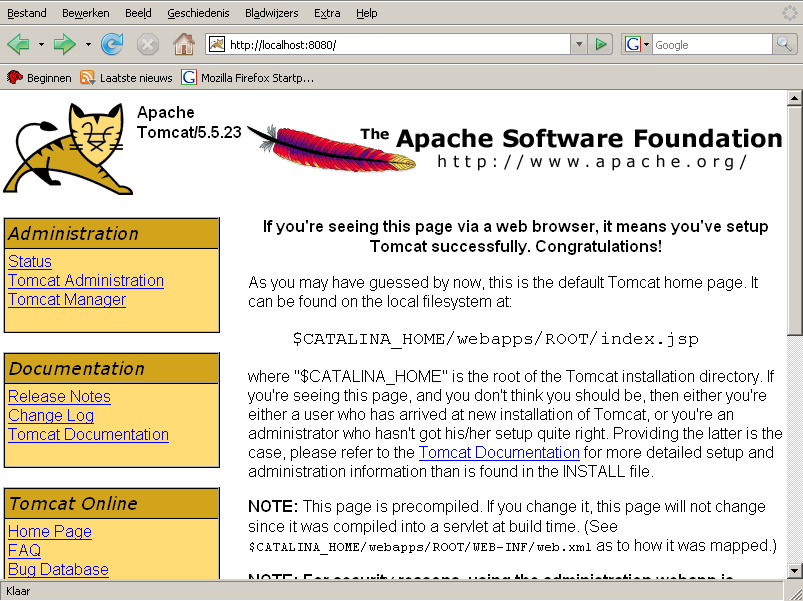
\includegraphics[width=8cm] {pics/nsis/tomcat_page.png}}
Navigate to the manager page and fill in the proper username and password.
\\
\vspace{0.5cm}~ \\ \centerline{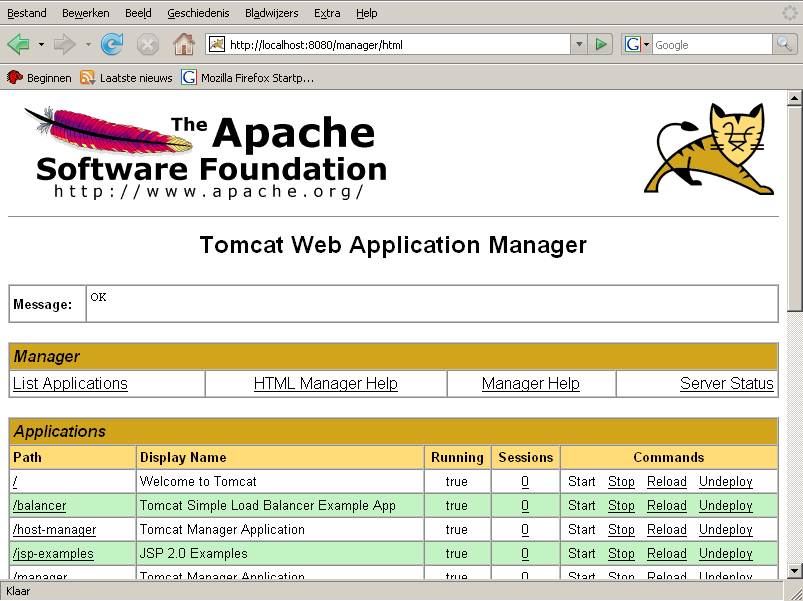
\includegraphics[width=8cm] {pics/nsis/tomcat_page_manager_1.png}}
Go to the Deploy section, browse for the regadb.war file and click \textbf{Deploy}. RegaDB will be deployed in the servlet container, this might take a few minutes.
\\
\vspace{0.5cm}~ \\ \centerline{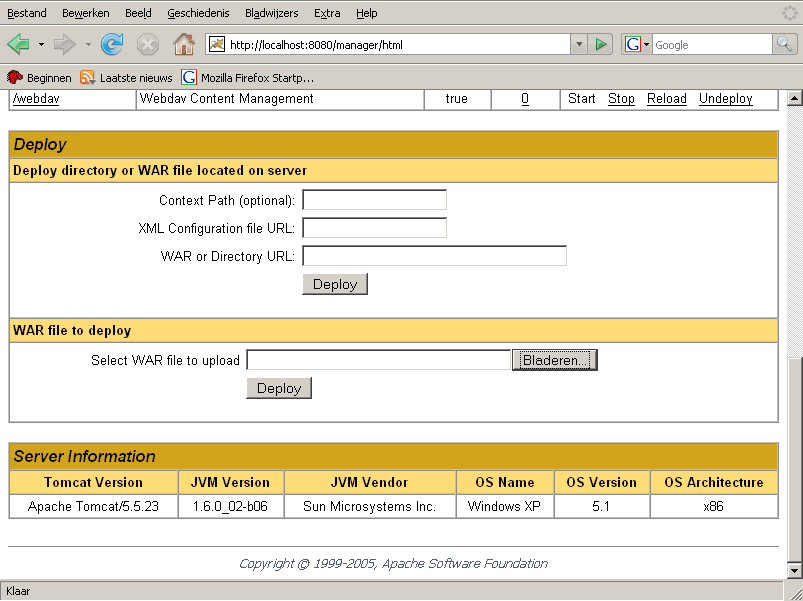
\includegraphics[width=8cm] {pics/nsis/tomcat_page_manager_2.png}}

\chapter{Post installation}
\label{chapter:post_install}

\section{Update RegaDB with the latest auxilary data}
Navigate your browser to \textit{http://localhost:8080/regadb/RegaDB}, and login to the system.
\\
\vspace{0.5cm}~ \\ \centerline{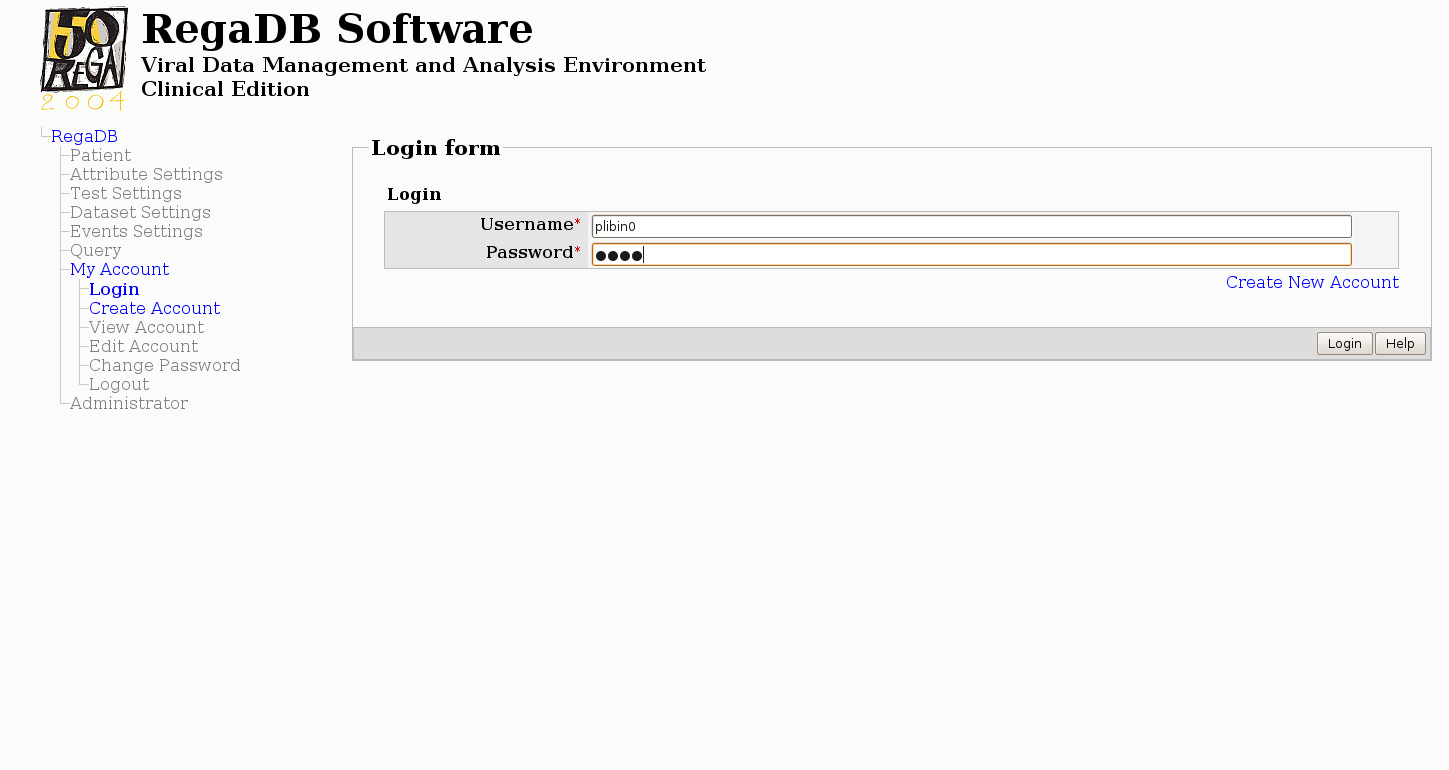
\includegraphics[width=15cm] {pics/auxilary/aux_1.png}}
\\
\vspace{0.5cm}~ \\ \centerline{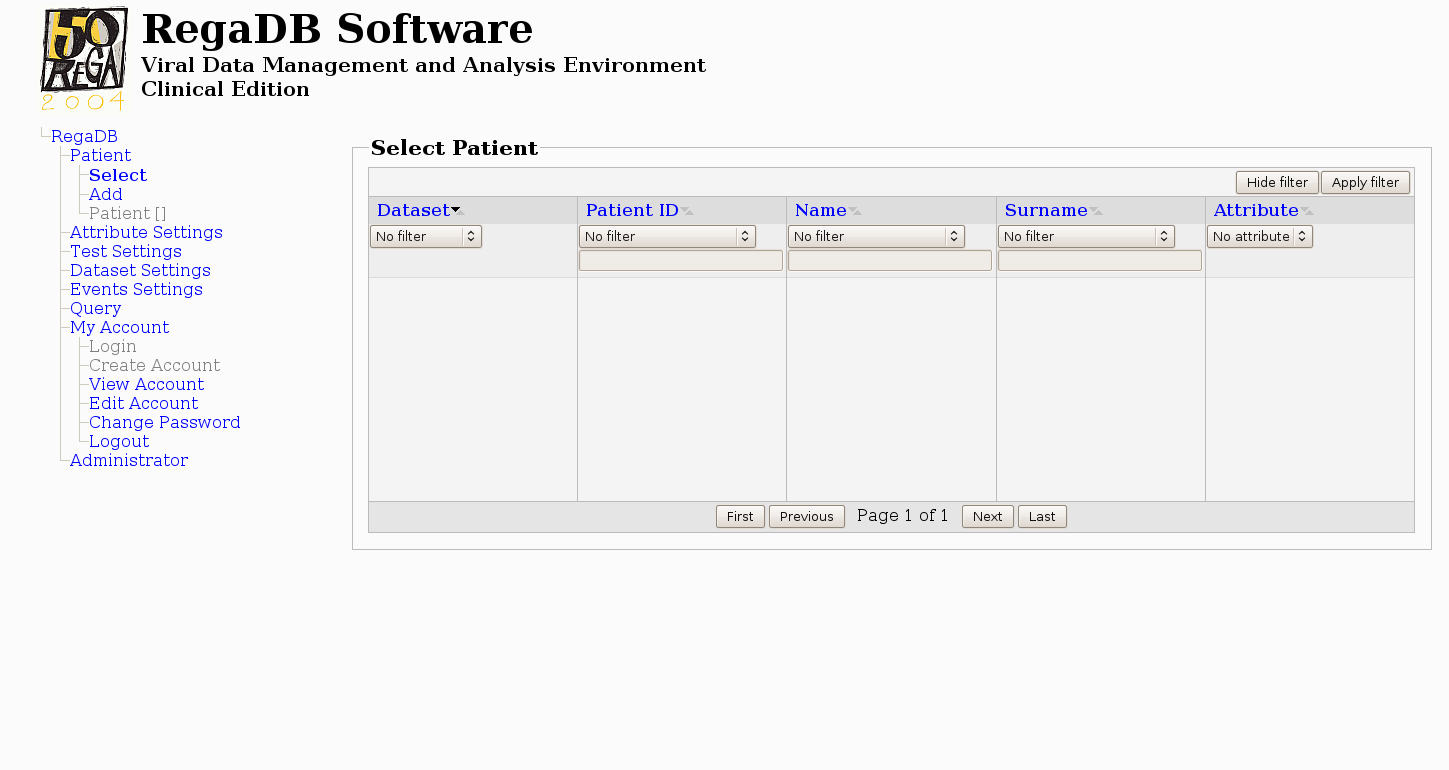
\includegraphics[width=15cm] {pics/auxilary/aux_2.png}}
\\
Navigate to the Administrator, Update from RegaDB Server page.
\\
\vspace{0.5cm}~ \\ \centerline{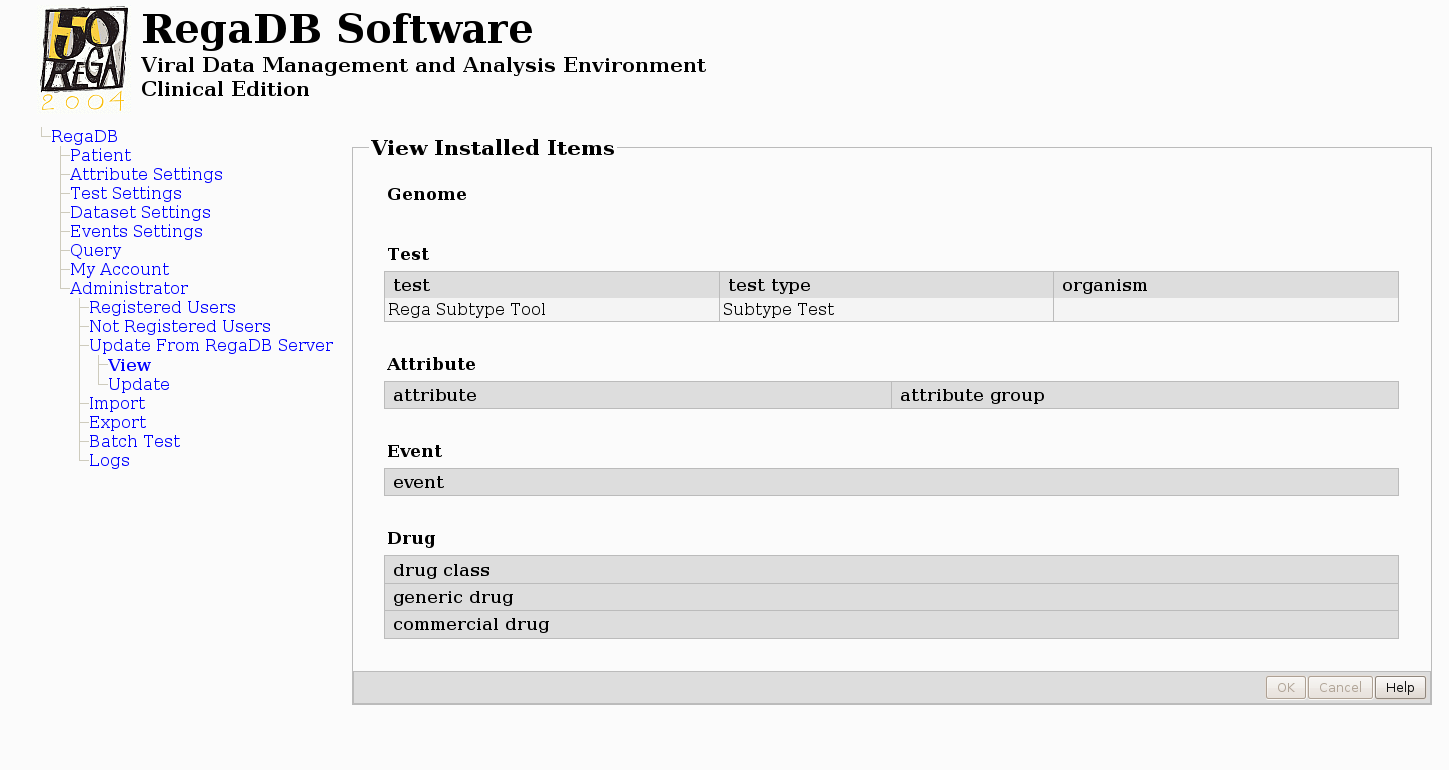
\includegraphics[width=15cm] {pics/auxilary/aux_3.png}}
\\
Click on Update, and a simulation update will be performed. This might take a few minutes, depending on your internet connection speed.
\\
\vspace{0.5cm}~ \\ \centerline{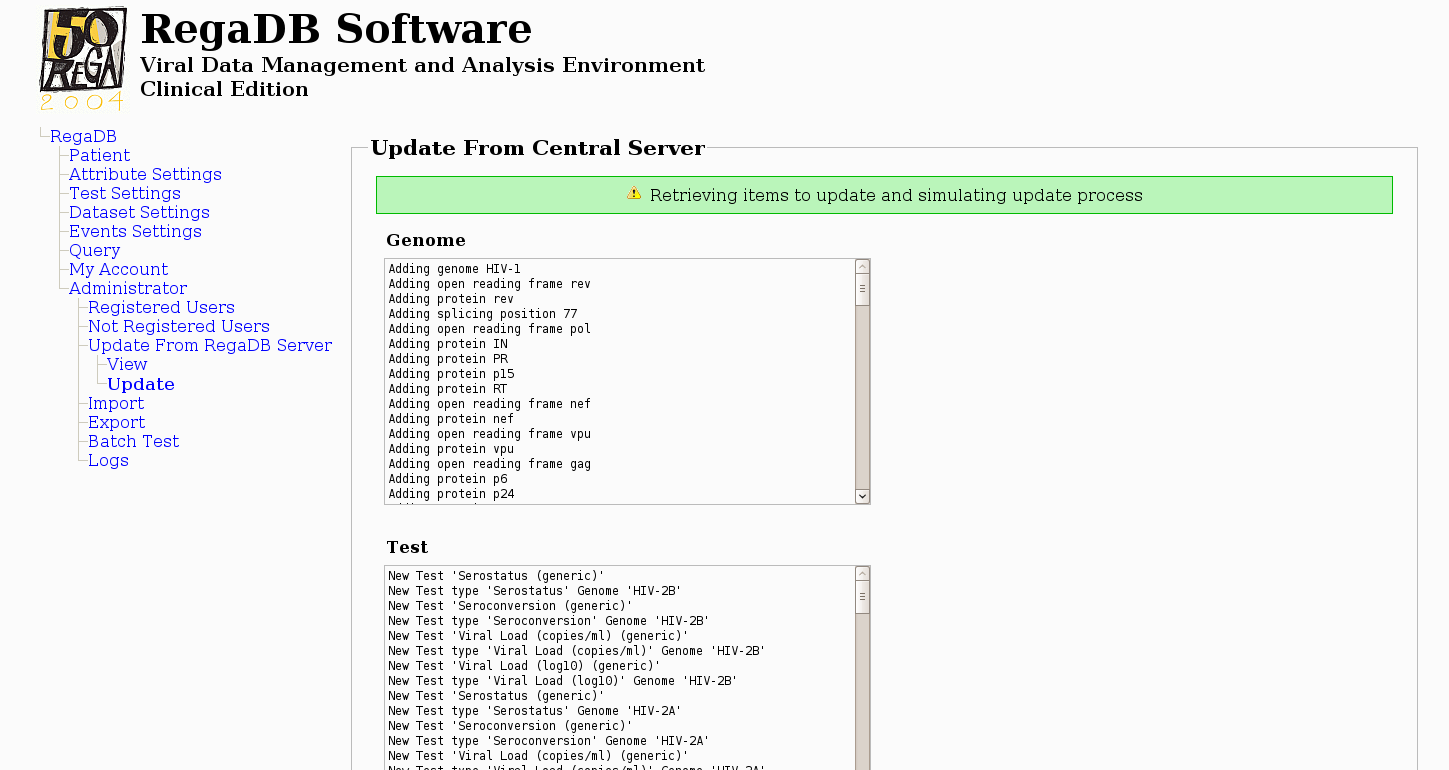
\includegraphics[width=15cm] {pics/auxilary/aux_4.png}}
\\
Click \textbf{OK} to confirm this simulation and to load the items into your local RegaDB instance. Again, this procedure might take a few minutes.
\\
\vspace{0.5cm}~ \\ \centerline{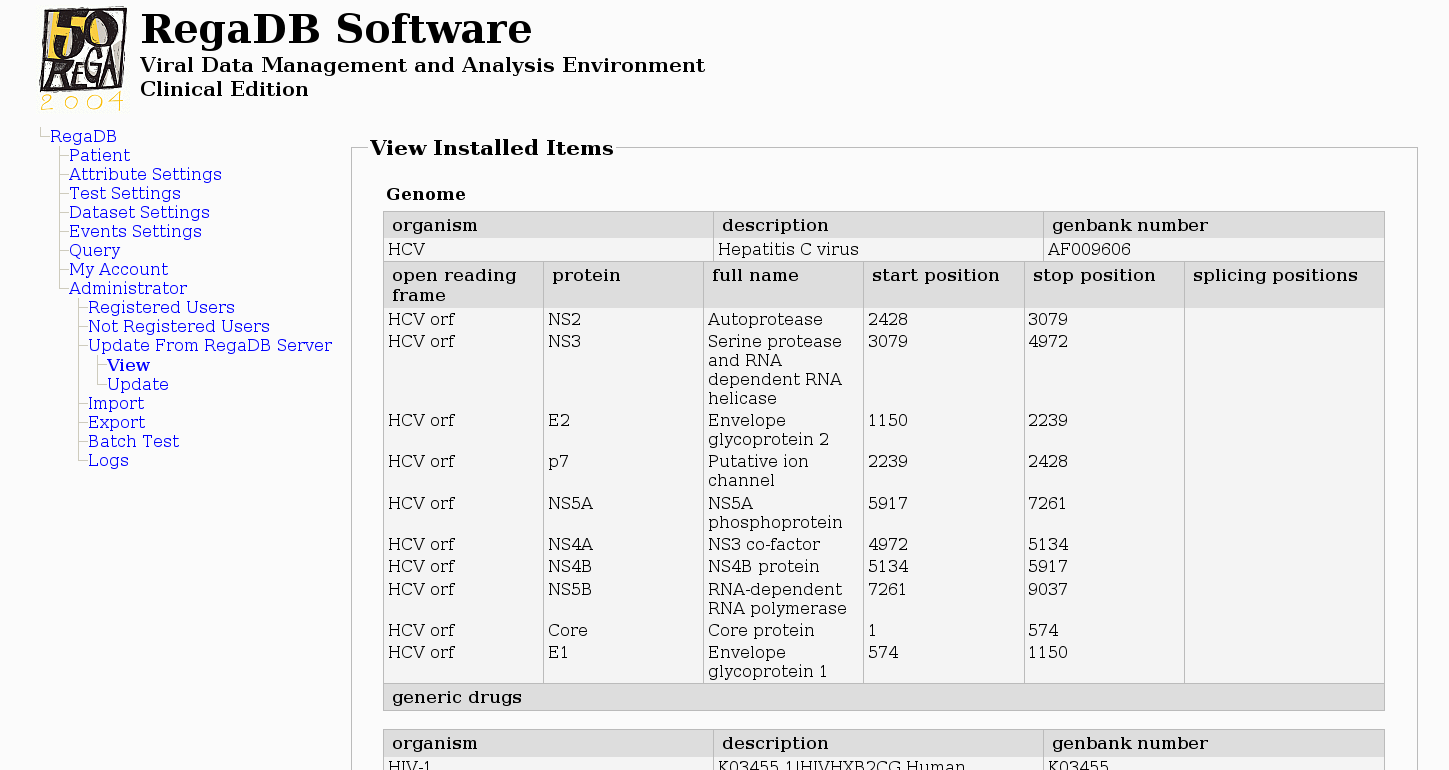
\includegraphics[width=15cm] {pics/auxilary/aux_5.png}}
\\
\section{Add a Dataset}
Navigate to the Administrator, Dataset settings menu, and add a new Dataset to the system.
\section{Contamination tool}
\subsection{Approximating distribution parameters}
The contamination tool uses both inter- and intra-patient sequence distance distributions. These distributions can be configured for multiple regions within a genome. Usually, using the precomputed values (such as offered on our website (TODO add link to our website)) is sufficient, however, it is also possible to esitimate these values on a existing database.
This is done by sampling a subset of all inter- and intra-patient sequence distances in the database, and afterwards fitting these distances on a log-normal distribution.

To sample the sequences distances for inter- or intra-patient run the SampleDistances program (located in regadb-analyses/src/net/sf/regadb/contamination/), this program accepts the following arguments:
\begin{itemize}
\item username 
\item password 
\item csv outputfile (eg.: outputfile.csv) 
\item outputType (intra-patient=I, inter-patient=O) 
\item ORF (eg.: pol) 
\item region range relative to the ORF (eg.: 169-1786) 
\end{itemize}

After sampling the distances, the approximation script can be used to fit the distances on a log-normal distribution. This script requires both an inter- and intra-patient distances csv file. The script can be found in regadb-analyses/src/net/sf/regadb/contamination and can be invoked with the following command and arguments:
\\
\textbf{Rscript regadb-analyses/src/net/sf/regadb/contamination/approximate\_distributions.R --intra intra.csv --inter inter.csv}


% include the index
%\cleardoublepage
%\addcontentsline{toc}{chapter}{section}{Index}
%\printindex

\end{document}
